\documentclass[10pt]{beamer}
\usepackage[utf8]{inputenc}
\usepackage{graphicx}

\usetheme{Madrid}
\usecolortheme{default}
\useinnertheme{circles}

\definecolor{Logo1}{rgb}{0.208, 0.2865, 0.373}
\definecolor{Logo2}{rgb}{0.000, 0.674, 0.863}

\setbeamercolor*{palette primary}{bg=Logo1, fg=white}
\setbeamercolor*{palette secondary}{bg=Logo2, fg=white}
\setbeamercolor*{palette tertiary}{bg=white, fg=Logo1}
\setbeamercolor*{palette quaternary}{bg=Logo1,fg=white}
\setbeamercolor{structure}{fg=Logo1} % itemize, enumerate, etc
\setbeamercolor{section in toc}{fg=Logo1} % TOC sections
\setbeamersize{text margin left=0.75cm,text margin right=0.75cm} 

\setbeamertemplate{bibliography item}{\insertbiblabel}

%------------------------------------------------------------
%This block of code defines the information to appear in the
%Title page
\setbeamerfont{title}{size=\large}
\title{Monocular Depth Estimation via Ensemble Deep Learning}

\author{Chinchuthakun Worameth}

\institute[]{
  Department of Transdisciplinary Science and Engineering\\
  Tokyo Institute of Technology
}

\date{\today}


\begin{document}

%The next statement creates the title page.
\frame{\titlepage}


%---------------------------------------------------------
%This block of code is for the table of contents after
%the title page
\AtBeginSection[]
{
    \begin{frame}
        \frametitle{Table of Contents}
        \tableofcontents[currentsection]
    \end{frame}
}
%---------------------------------------------------------

\section{Introduction}

%---------------------------------------------------------
%Changing visivility of the text
\begin{frame}{What is monocular depth estimation?}

\begin{itemize}
    \item Predict depth information/generating a corresponding \textbf{depth map} from images or a video sequence of a single camera
    \item Provide a cost, space, and energy efficient alternative to existing depth sensors, e.g. LiDARs which are large and have high power consumption, especially in small robotic platforms.
\end{itemize}
\smallskip
\begin{columns}
    \begin{column}{.45\linewidth}\centering
    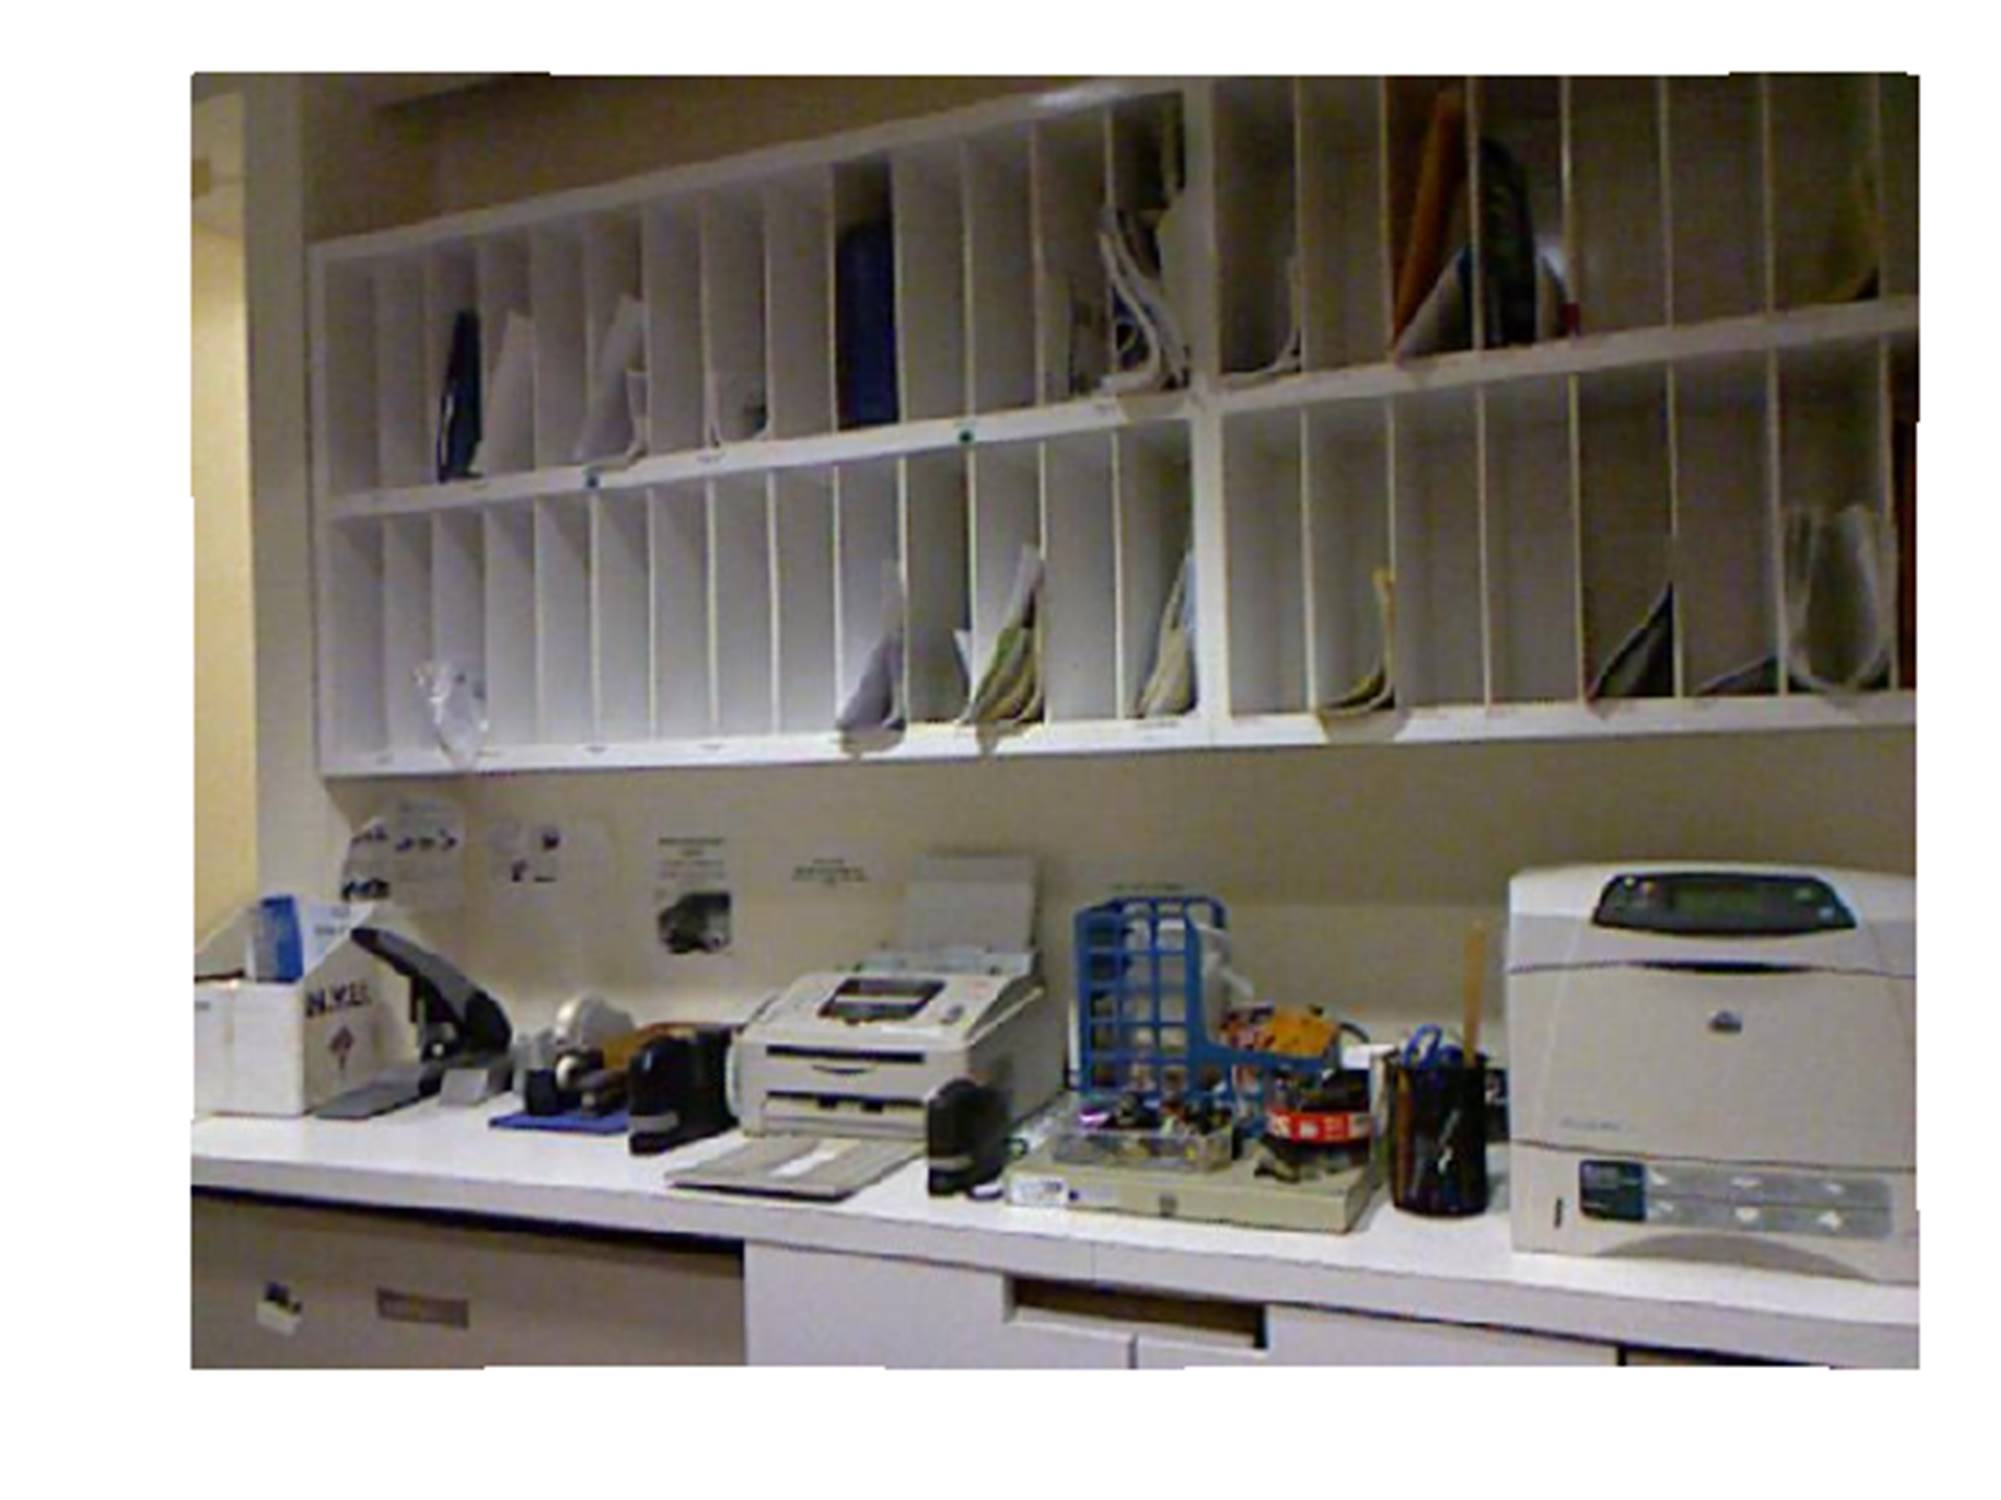
\includegraphics[width=5.3cm]{depthmap_real.jpg}\par
    Raw image
    \end{column}
    \begin{column}{.45\linewidth}\centering
    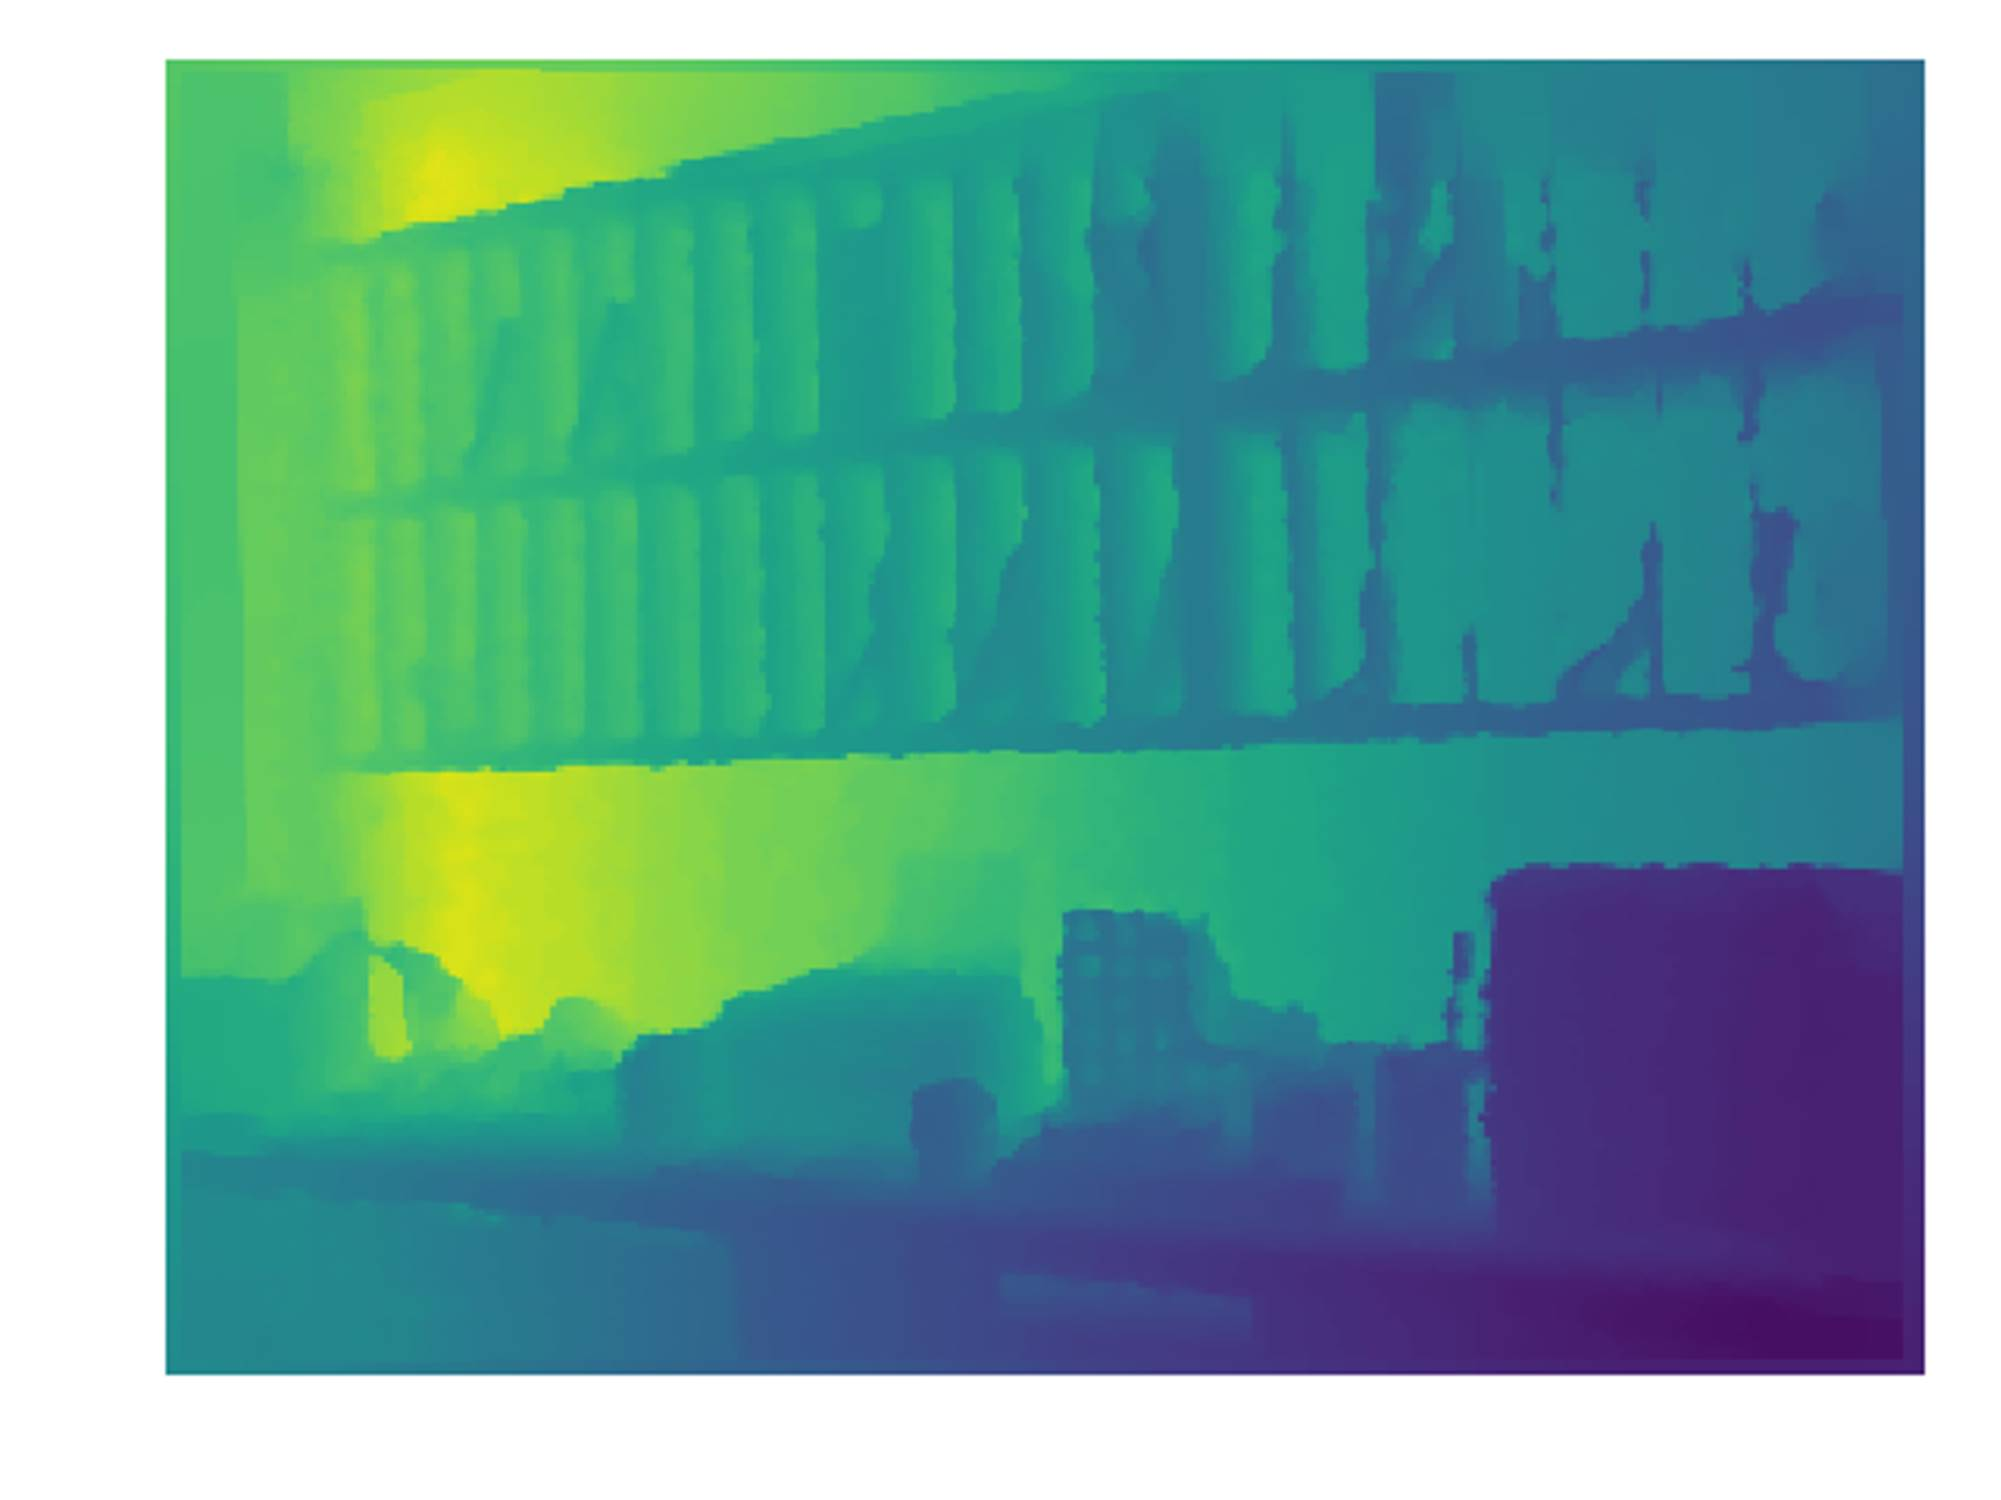
\includegraphics[width=5.3cm]{depthmap_depth.jpg}\par
    Depth map
    \end{column}
\end{columns}
\end{frame}

\section{Literature Review}

\begin{frame}{Monocular Depth Estimation at a glance}
    Deep learning approaches are classified into 3 main types:
    \begin{itemize}
        \item \textbf{Supervised}: Use ground truth depth maps and frame the problem as a regression one
        \item \textbf{Unsupervised}: Exploit geometric constraints between frames in monocular video sequence
        \item \textbf{Semi-supervised}: Basically unsupervised approach with known transformation between frames
    \end{itemize}
    
    \vspace{0.3cm}
    
    Current challenges in the field include, but not limited to, the followings:
    \begin{itemize}
        \item \textbf{Accuracy}: as a matter of course, especially in unsupervised methods
        \item \textbf{Transferability}: train on one dataset, test on another
        \item \textbf{Real-time Performance}: lightweight and low-latency networks
    \end{itemize}
\end{frame}

\begin{frame}{FastDepth: Fast Monocular Depth Estimation on Embedded Systems}
    This paper proposes a lightweight decoder for monocular depth estimation with details summarized as follows:
    \begin{itemize}
        \item Contains only \textbf{depthwise separable convolutions}
        \item When decoding, interpolate \textbf{after} convolution instead of before
    \end{itemize}
    While it has low-latency and smaller size (even smaller after network pruning), its accuracy is naturally worse than state of the arts.
    
    \vspace{0.3cm}    
    \centering
    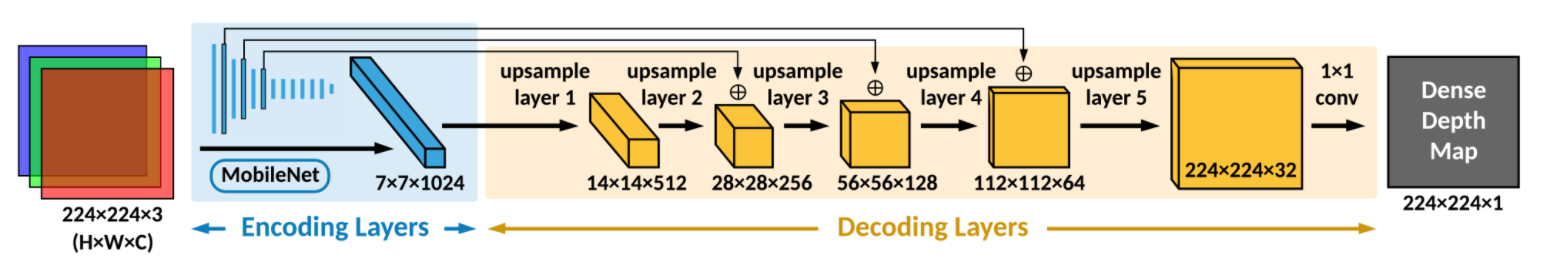
\includegraphics[width=11cm]{fastdepth_architecture.png}\par
    FastDepth Architecture \cite{fastdepth}
\end{frame}
    
\begin{frame}{Supplementary \#1: Depthwise Separable Convolution}
    \centering
    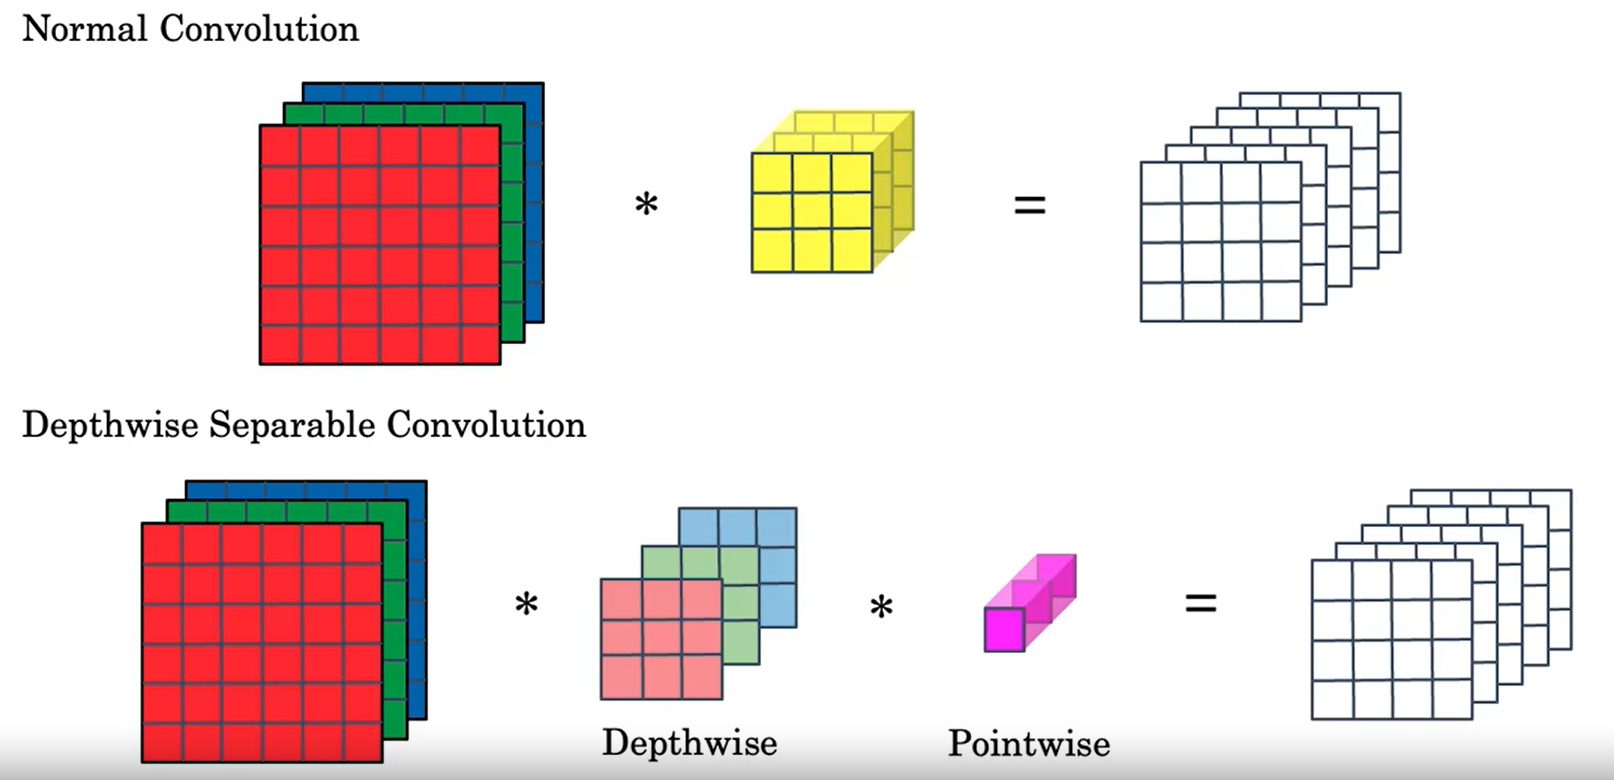
\includegraphics[width=11cm]{DSconv.png}\par
    Computational cost comparison
\end{frame}

\begin{frame}{Supplementary \#2: Why Interpolation + Convolution instead of Transpose convolution}
    \centering
    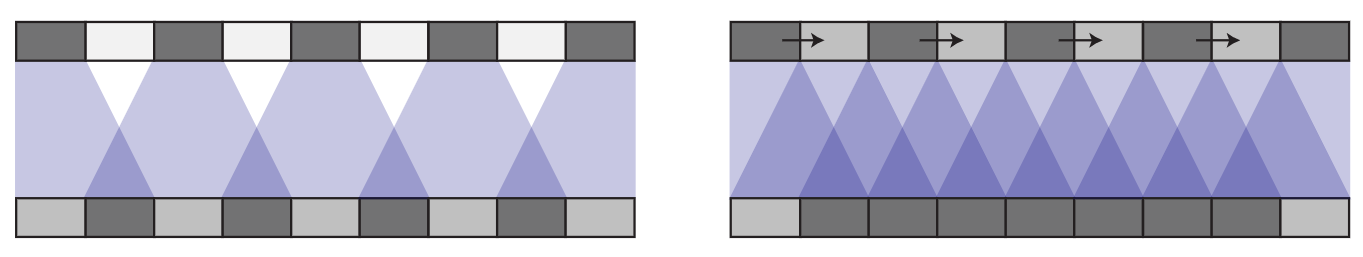
\includegraphics[width=8cm]{TransposeConv2.png}\par
    Coverage of Transpose Conv (left) and Conv + Int (right)
    
    \centering
    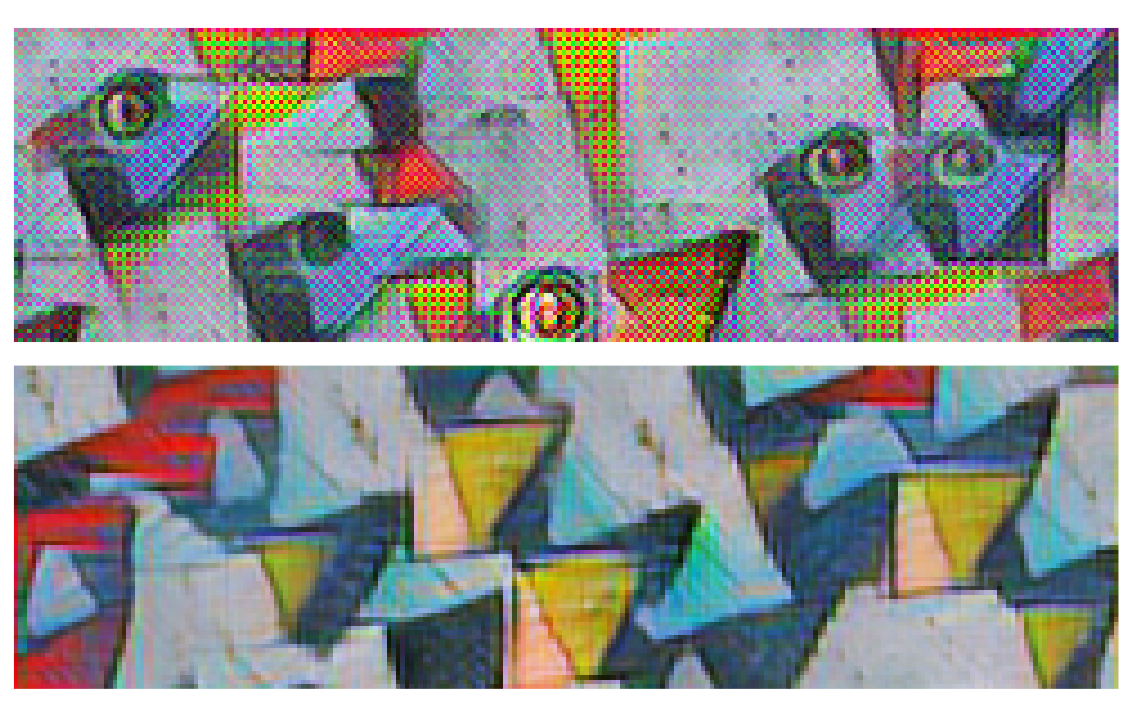
\includegraphics[width=6cm]{TransposeConv.PNG}\par
    Checker board patterns
\end{frame}

\begin{frame}{BTS: From Big to Small: Multi-Scale Local Planar Guidance for Monocular Depth Estimation}
    \centering
    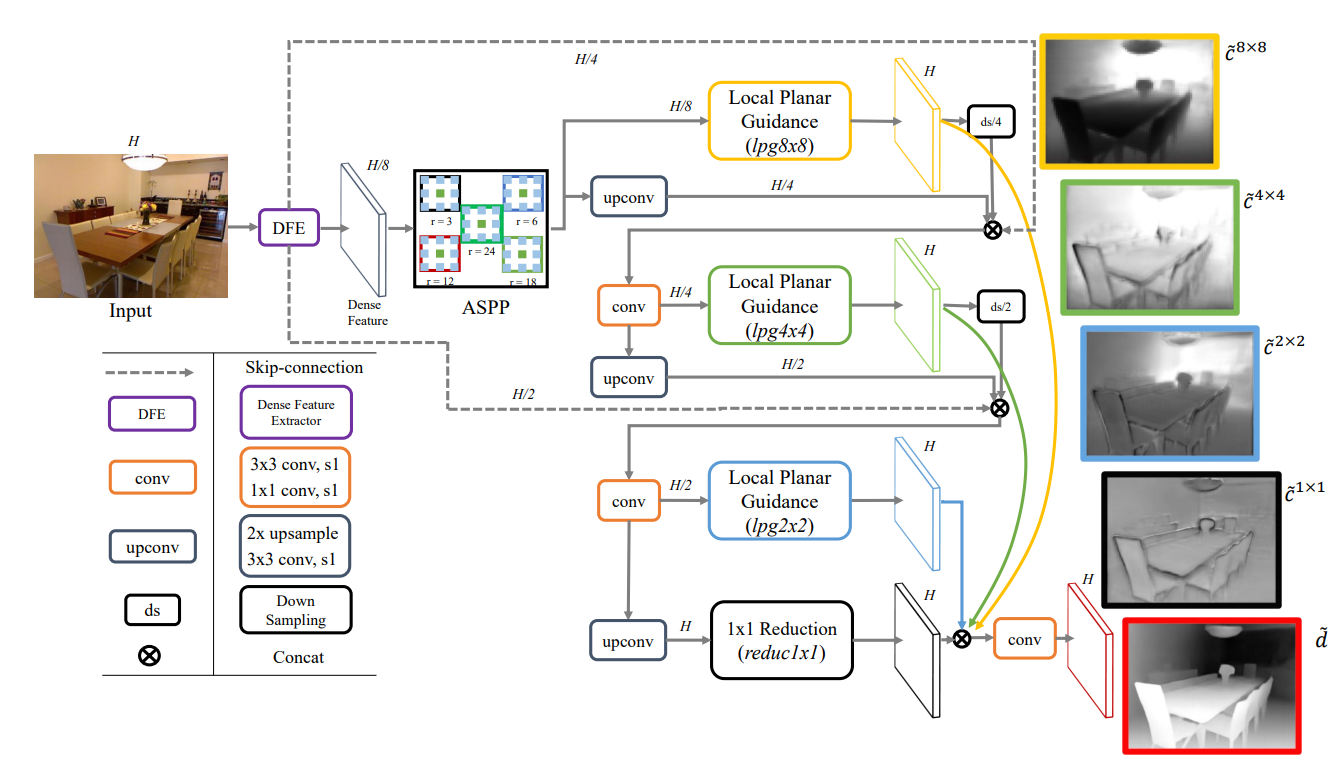
\includegraphics[width=10cm]{bts_architecture.png}\par
    BTS architecture \cite{bts}
\end{frame}

\begin{frame}{AdaBins: Depth Estimation using Adaptive Bins}
    \begin{itemize}
        \item Rephrase the problem to multi-class classification one by quantizing depth values into bins to obtain discrete depth values
        \item Bin width is automatically adjusted for each image by a visual-transformer network (ViT)
        \item Final depth values are computed by a linear combination of bin centers to suppress discretization artifacts
    \end{itemize}
    \smallskip
    \centering
    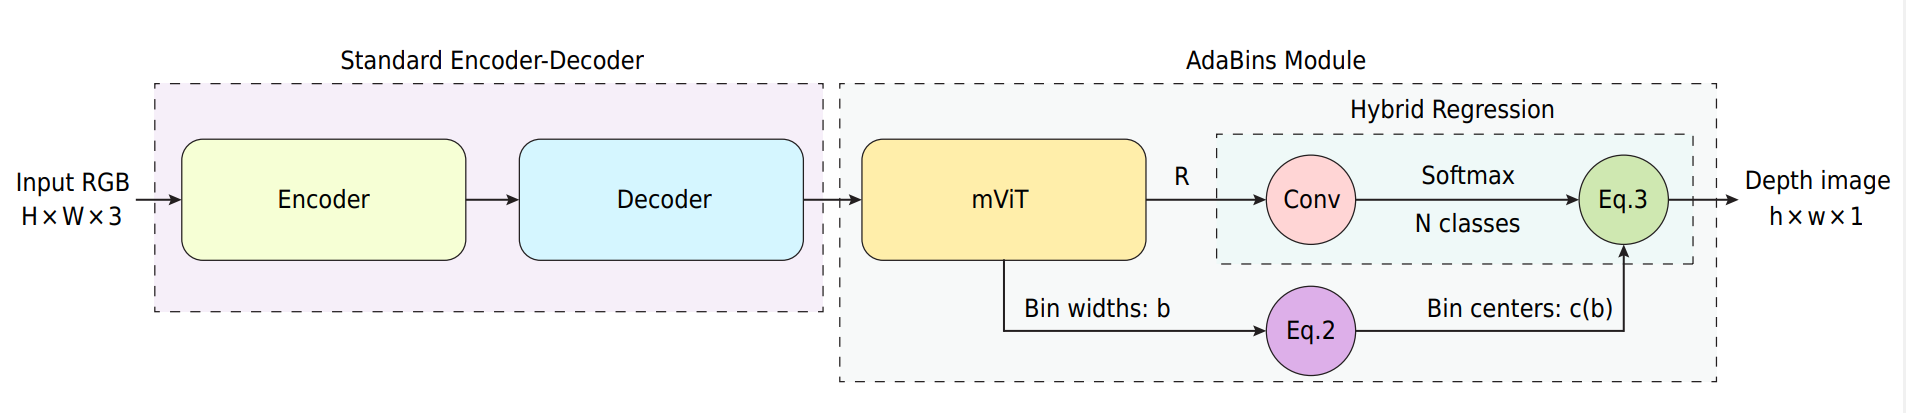
\includegraphics[width=11cm]{adabins_architecture.png}\par
    Adabins architecture \cite{adabins}
\end{frame}

\begin{frame}{Ensemble Deep Learning}
    \textbf{Ensemble deep learning} refers to an approach of combining prediction of multiple neural networks to make final decision. While it has been applied in different tasks, e.g. image classification and text summarization, a recent survey indicates no application in monocular depth estimation.
    
    \vspace{0.3cm} 
    \centering
    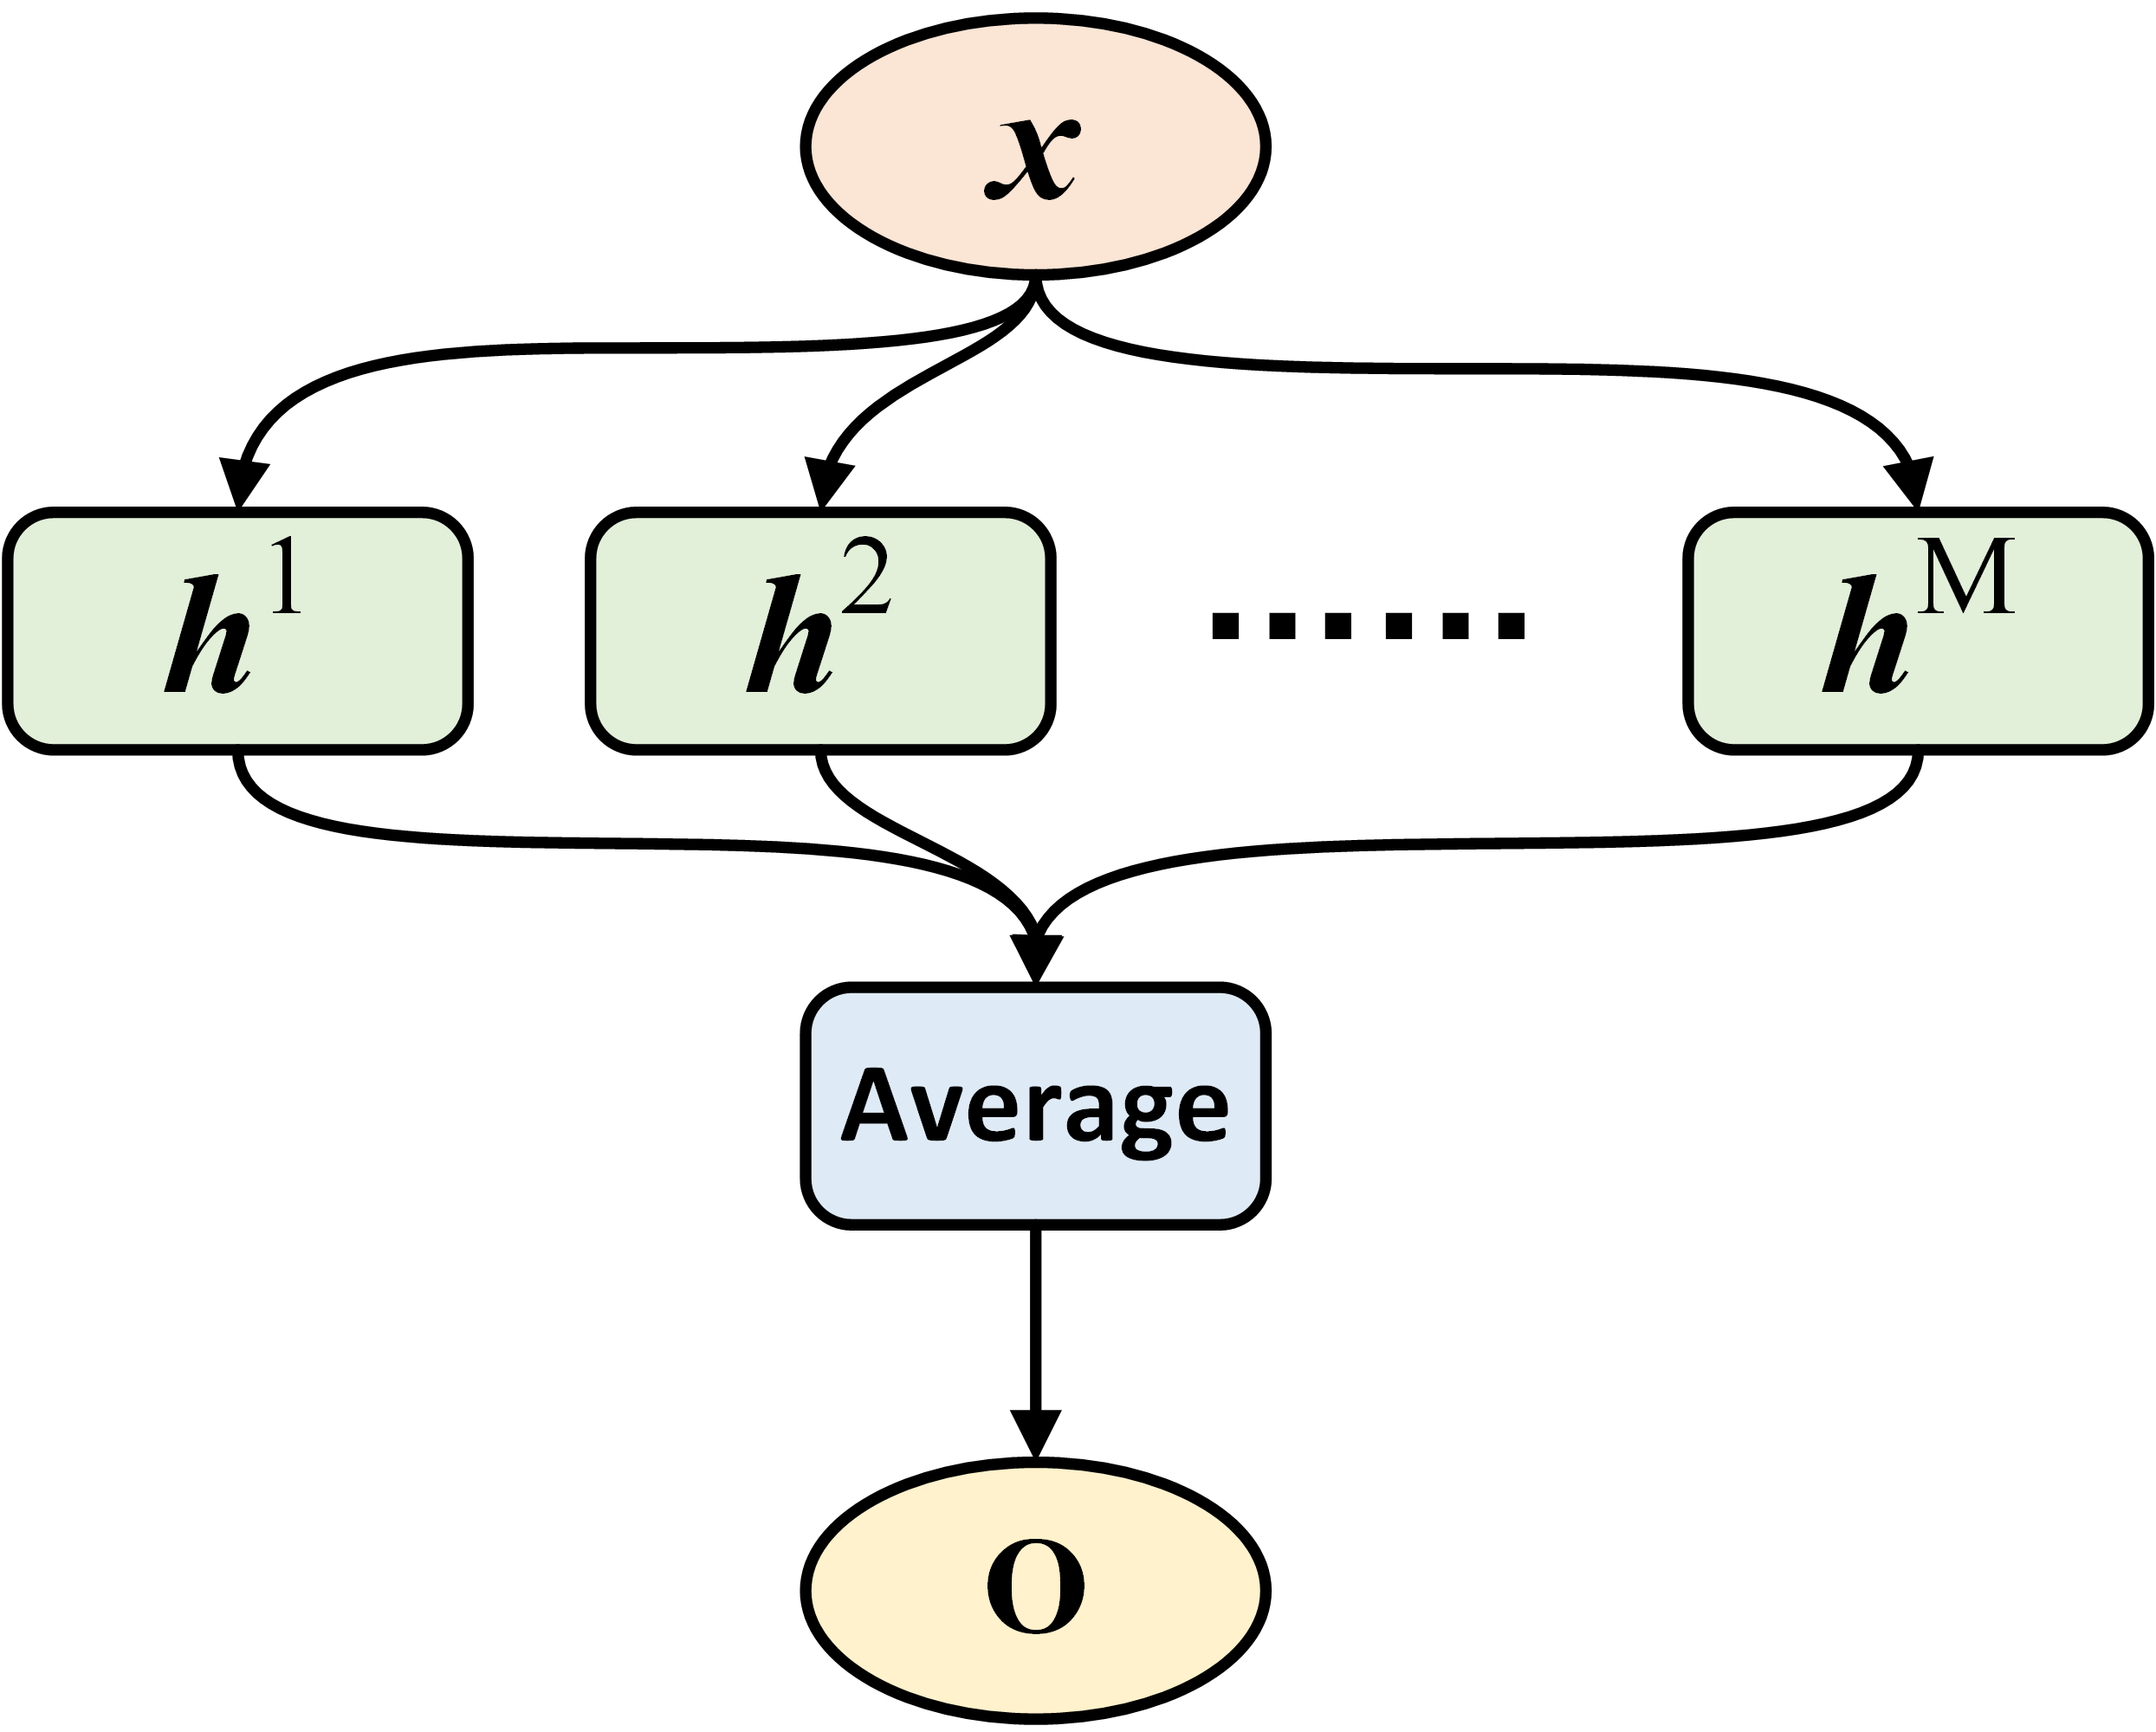
\includegraphics[width=5cm]{ensemble_fusion.png}\par
    Fusion and Voting Paradigm
\end{frame}

\section{Research Proposal}
\begin{frame}{Objective}
    \textbf{Currently, aiming to}:
    \begin{itemize}
        \item Demonstrate prospect application of ensemble deep learning in Monocular Depth Estimation by reaching (approximately) the same level of performance with the \textbf{downgraded} version of the original models, \textbf{consisting of less than half of parameters}.
    \end{itemize}
    
    \vspace{0.3cm} 
    
    \textbf{If possible}:
    \begin{itemize}
        \item Exceed the original model's performance (This is likely not possible since \textbf{both models are one of the most recent SOTAs in KITTI and NYU V2 dataset})
    \end{itemize}
    
\end{frame}

\begin{frame}{Proposed Method: Overview}
    \begin{itemize}
        \item Consists of Adabins \cite{adabins} and BTS \cite{bts}
        \item Partly inspired by FastDepth \cite{fastdepth}, Adabins and BTS are simplified (reduce number of parameters) by
            \begin{itemize}
                \item Use GhostNet \cite{ghostnet}, pretrained by ImageNet, as the encoder
                \item When upsampling feature maps, interpolate after convolution
                \item Substitute convolutions by depthwise seperable convolutions
            \end{itemize}
        \item Final prediction is the mean of output depth map of each model
        \item Number of parameters:
            \begin{itemize}
                \item \textbf{Original BTS}: 47.0M
                \item \textbf{Original Adabins}: 78.2M
                \item \textbf{Proposed Ensemble}: 26.3M
            \end{itemize}
    \end{itemize}
\end{frame}

\begin{frame}{Supplementary \#3: GhostNet: More Features from Cheap Operations \cite{ghostnet}}
    \begin{itemize}
        \item Based on observation that the output feature maps of convolutional layers often contain much redundancy
        \item Generate some feature maps through usual convolution. Then, apply \textbf{linear operations} to generate more feature maps
        \item \textbf{GhostNet} is obtained by arranging \textbf{ghost modules} in a structure similar to MobileNetV2
    \end{itemize}
    
    \centering
    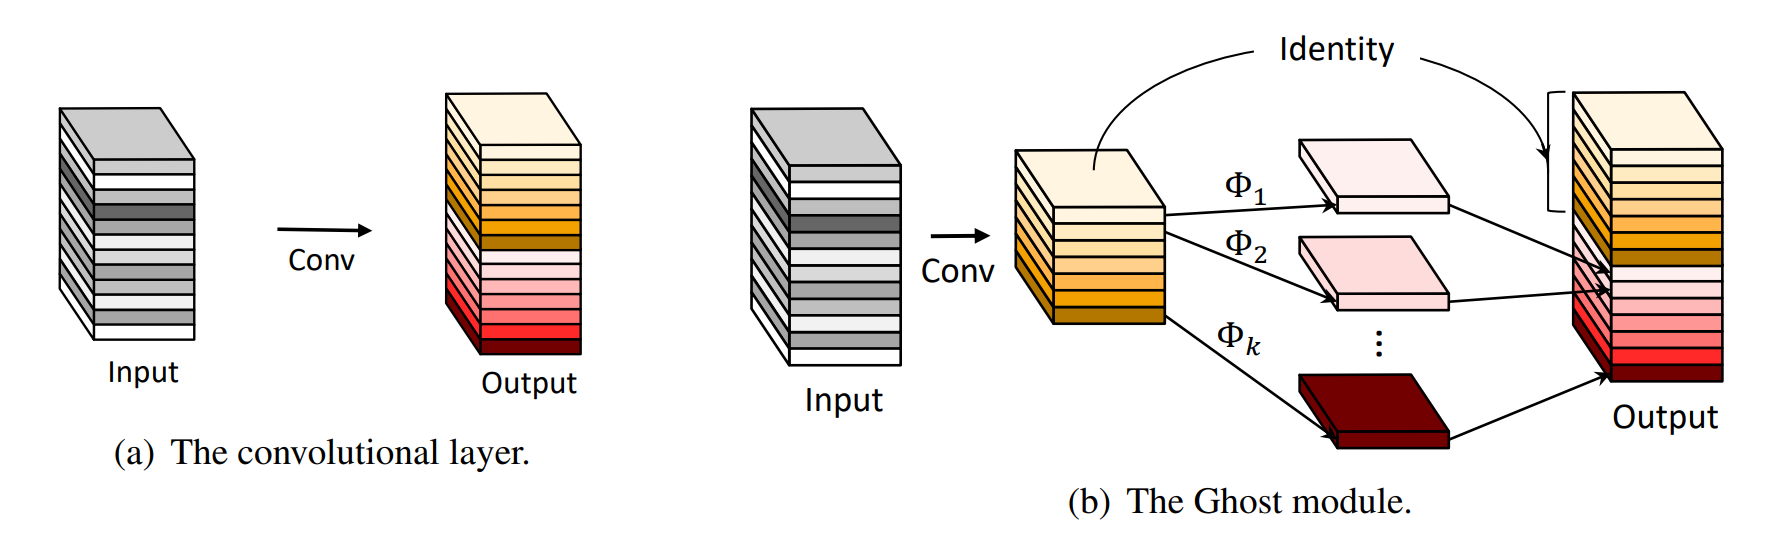
\includegraphics[width=9cm]{ghost_module.png}\par
    Ghost module \cite{ghostnet}
\end{frame}

\begin{frame}{Proposed Method: Loss functions}
    Similar to \cite{adabins}, \textbf{pixel-wise depth loss} and \textbf{bin-center density loss} are used to mitigate pixel-wise difference and encourage the distribution of bin centers to follow the distribution of depth values in the ground truth, respectively. Since \cite{bts} also uses pixel-wise depth loss, both sub-networks are trained simultaneously using a loss function defined by:
    
    \vspace{0.1cm} 
    
    $$L_{\text{total}}=L_{\text{pixel}}+L_{\text{bins}}$$
    $$L_{\text{pixel}}=\alpha\sqrt{\frac{1}{N}\sum_{i=1}^{N}y_i^2-\frac{\lambda}{N^2}(\sum_{i=1}^{N}y_i)^2}$$
        where $y_i^{2}=\log(d_i)-\log(d_i^{*})$ and $d_i^{*}$ is ground truth depth
    $$L_{\text{bins}}=\textbf{BiChamfer}(c(b),D)+\textbf{BiChamfer}(D,c(b))$$
    
    \vspace{0.1cm} 
    
    Note that $\lambda=0.85$ and $\alpha=10$ are used as same as the original Adabins \cite{adabins}
    
\end{frame}

\begin{frame}{Evaluation: Datasets and Data Augmentation}

    NYU Depth V2 and KITTI, are used to evaluate the performance:
    \begin{itemize}
        \item \textbf{NYU Depth V2}: indoor scenes, acquired from a RGB-D camera. Training data are extracted in the same manner as \cite{bts} and \cite{adabins}
        \item \textbf{KITTI}: outdoor scenes, acquired from LiDARs
    \end{itemize}
    
    \vspace{0.3cm} 
    
    Similar to \cite{bts} and \cite{adabins}, the following augmentation are applied to avoid overfitting:
    \begin{itemize}
        \item \textbf{Random horizontal flipping} with probability of 0.5
        \item \textbf{Random contrast, brightness, and color adjustment} in a range of [0.9, 1.1] with probability of 0.5
        \item \textbf{Random crop} of size $416\times544$ for NYU V2 and $352\times704$ for KITTI
        \item \textbf{Random rotation} of degree in ranges of [-2.5,2.5] for NYU V2 and [-1,1] for KITTI
    \end{itemize}
\end{frame}

\begin{frame}{Supplementary \#4: KITTI dataset}
\begin{itemize}
    \item Consists of 56 different outdoor scenes
    \item Official split is 28 for training and 28 for testing
    \item Constructed by stereo image pairs and ground truth depth obtained from LIDAR
\end{itemize}

\smallskip
\centering
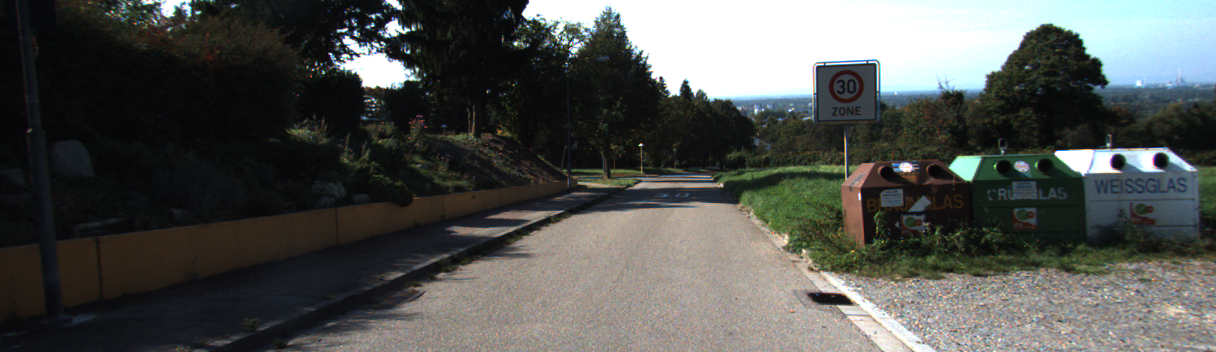
\includegraphics[width=10cm]{kitti_sample.png}\par
A sample of raw image from KITTI dataset

\end{frame}

\begin{frame}{Supplementary \#5: NYU Depth V2 dataset}
\begin{itemize}
    \item Consists of 464 different indoor scenes
    \item Official split into is for training and 215 for testing
    \item Constructed by monocular video sequences of scenes and ground truth of depth captured by an RGB-D camera
\end{itemize}

\smallskip
\centering
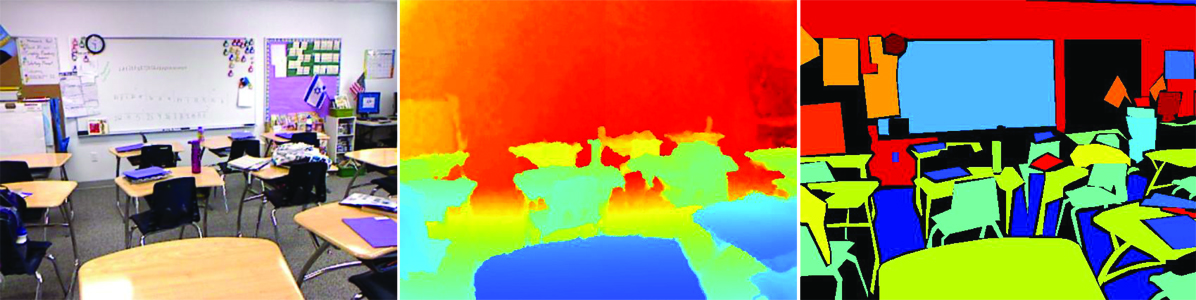
\includegraphics[width=10cm]{nyu_sample.jpg}\par
A sample of raw image, preprocessed depth, and labeled from the dataset

\end{frame}

\begin{frame}{Evaluation: Metrics}
    Standard metrics used in previous works include:
    \begin{itemize}
        \item \textbf{Threshold Accuracy}: $\%$ of $d_i$ s.t. $\text{max}\Big(\frac{d_i}{d_i^{*}},\frac{d_i^{*}}{d_i}\Big)=\delta<\text{threshold}$, usually threshold $=1.25,1.25^2,1.25^3$
        \item \textbf{Average Relative Error (REL)}: $\frac{1}{N}\sum\Big(\frac{\lvert d_i-d_i^{*}\rvert}{d_i^{*}}\Big)$
        \item \textbf{Root Mean Squared Error (RSME)}: $\sqrt{\frac{1}{N}\sum( d_i-d_i^{*})^{2}}$
        \item \textbf{Average $\log_{10}$ Error}: $\frac{1}{N}\sum\lvert \log_{10}(d_i)-\log_{10}(d_i^{*}) \rvert$
        \item \textbf{Squared REL (Sq REL)}: $\frac{1}{N}\sum\frac{\Vert d_i-d_i^{*}\Vert}{d_i^{*}}$
        \item \textbf{RSME of logarithm (RSME log)}: $\sqrt{\frac{1}{N}\sum\Vert \log d_i-\log d_i^{*}\Vert^{2}}$
    \end{itemize}
    
    \vspace{0.3cm}
    
    % Additionally, another two standard metrics are included for KITTI dataset:
    % \begin{itemize}
    %     \item \textbf{Squared REL (Sq REL)}: $\frac{1}{N}\sum\frac{\Vert d_i-d_i^{*}\Vert}{d_i^{*}}$
    %     \item \textbf{RSME of logarithm (RSME log)}: $\sqrt{\frac{1}{N}\sum\Vert \log d_i-\log d_i^{*}\Vert^{2}}$
    % \end{itemize}
    
\end{frame}

\begin{frame}{Proposed Method: Implementation}
    \begin{itemize}
        \item Implemented in \textbf{Pytorch}, trained in a Laboratory's server (Rat) using distributed training.
        \item \textbf{AdamW optimizer} \cite{adamw} together with \textbf{1-cycle policy} \cite{super-convergence} are used to train the model for fast convergence
        \item Maximum learning rate is determined from \textbf{lr range test} \cite{cyclical-lr}. \textbf{Batch size} is set to as large as possible, limited only by physical memory, to enable larger learning rate, as suggested by \cite{super-convergence}.
        \item Other hyperparameters are tuned via \textbf{grid search} and \textbf{random search} together with \textbf{Hyperband} \cite{hyperband}.
        \item Training and hyperparameter tuning are monitored by \textbf{Weights and Biases} platform
    \end{itemize}
    
\end{frame}

\begin{frame}{Result and Discussion (so far)}
    \begin{itemize}
        \item The model is evaluated on pre-defined center cropping, without other transformations, as described in \cite{eigen}
        \item At test time, the final output is the average of an image’s prediction and the prediction of its mirror image which is commonly used in previous work such as \cite{adabins}
    \end{itemize}
    
    

    \begin{table}[]
        \begin{tabular}{|c|c|c|c|c|}
        \hline
        \textbf{Metrics} & \textbf{BTS} & \textbf{Adabins} & \textbf{Proposed} \\ \hline
        Alpha1           & 0.885        & 0.903            & 0.851   \\ \hline
        Alpha2           & 0.978        & 0.984            & 0.973  \\ \hline
        Alpha3           & 0.994        & 0.997            & 0.993   \\ \hline
        REL              & 0.110        & 0.103            & 0.122  \\ \hline
        RMSE             & 0.392        & 0.364            & 0.450    \\ \hline
        log10            & 0.047        & 0.044            & 0.053    \\ \hline
        \end{tabular}
    \end{table}\par
    \centering
    Current best performance of proposed method on NYU Depth V2 dataset
    
\end{frame}

\begin{frame}{Result and Discussion (so far)}
    \begin{itemize}
        \item Varying momentum and learning rate did not yield significant improvement
        \item Does not seem to be overfitting
        \item So, what wrong? Global optima? Local optima? Saddle point?
    \end{itemize}
    \centering
    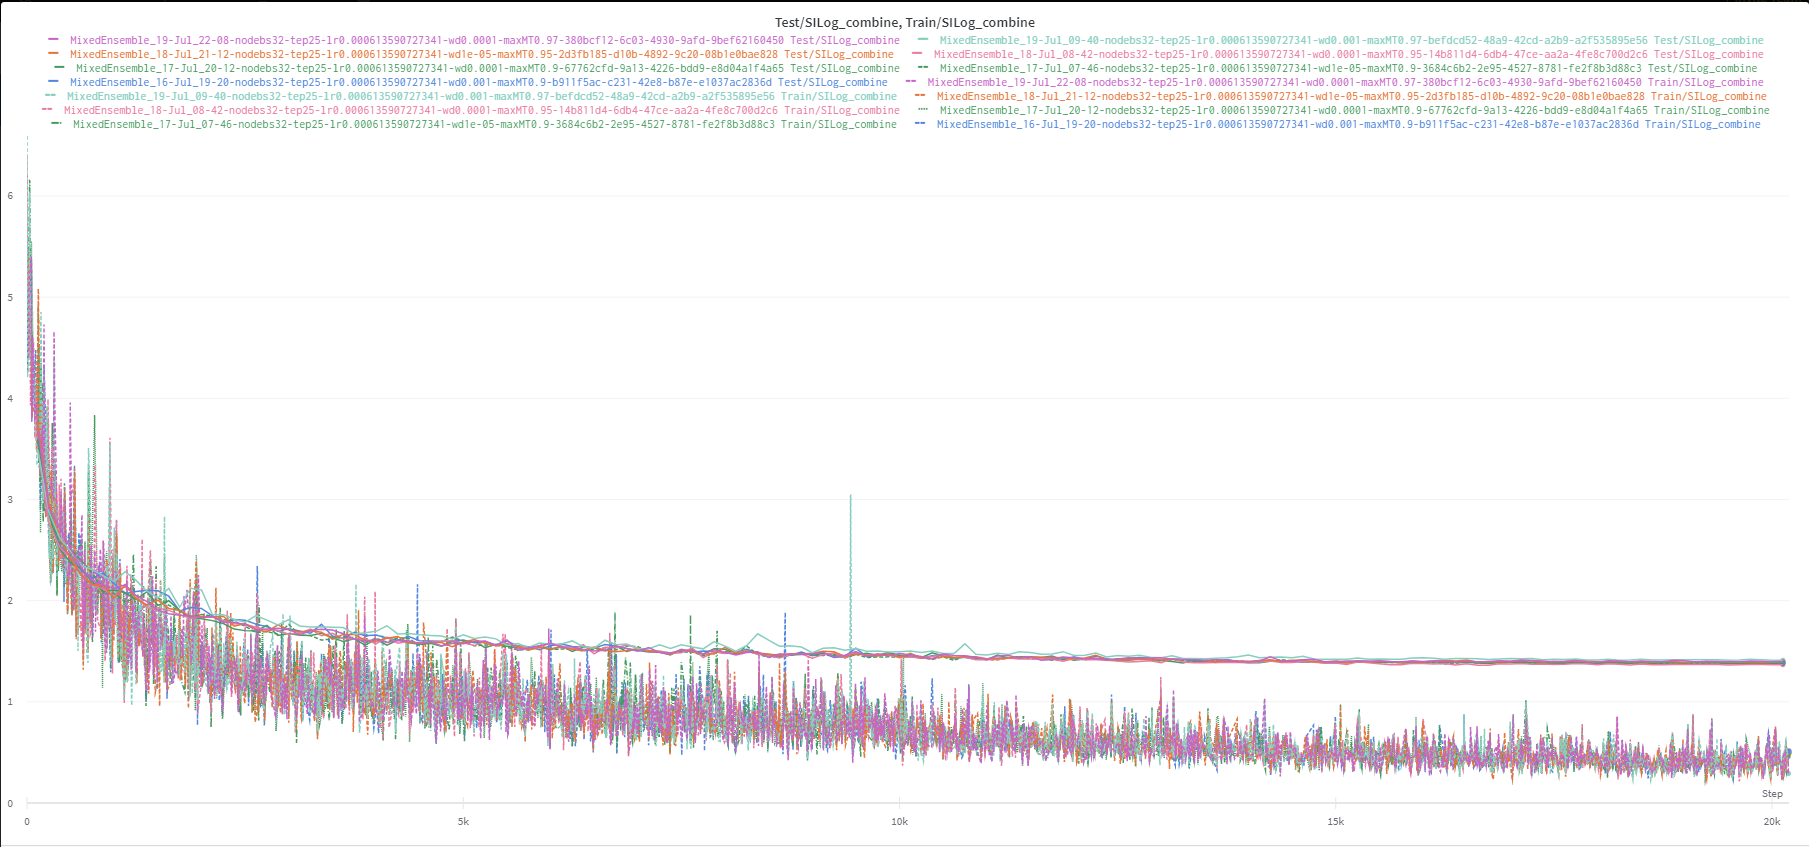
\includegraphics[width=11cm]{sweep_result.png}
\end{frame}

\begin{frame}{Result and Discussion (so far)}
    \begin{itemize}
        \item Increasing batch size and learning rate yields faster convergence
        \item Currently training, but probably no significant improvement, again...
    \end{itemize}
    \centering
    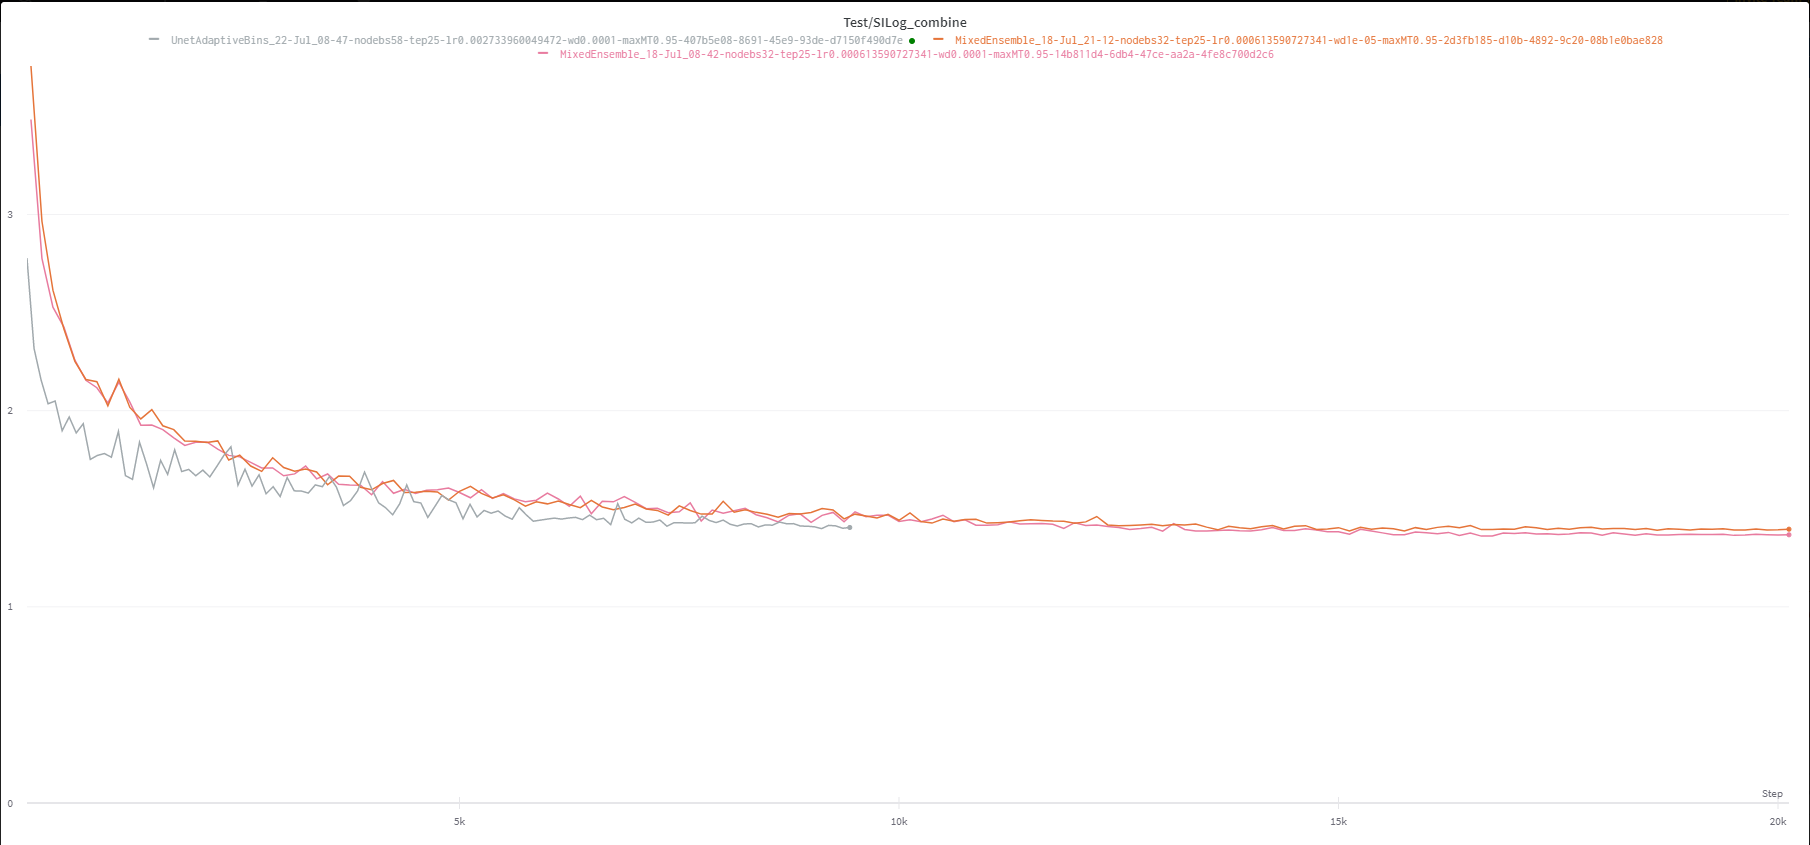
\includegraphics[width=11cm]{result_diff_bs-lr.PNG}
\end{frame}

\begin{frame}[t]{Future Works}
    \begin{itemize}
        \item \textbf{Implementation}
        \begin{itemize}
            \item Continue tuning hyperparameters
            \item Train and evaluate on KITTI dataset
        \end{itemize}
        \item \textbf{Design}
        \begin{itemize}
            \item Explore new strategies to regularize the training
            \item Continue tuning hyperparameters
        \end{itemize}
    \end{itemize}
\end{frame}

\begin{frame}[t, noframenumbering]{References}
    \scriptsize
    \nocite{*}
    \bibliographystyle{ieeetr}
    \bibliography{citations.bib}
\end{frame}

\end{document}